\subsubsection{Q10.20 data 10312021 grouped by scenario}

\begin{comment}
               EFPR        EO      EFNR     n    pvalue
(frauth,)  0.500000  0.500000  0.428571  21.0  0.898120
(icu,)     0.710526  0.289474  0.605263  19.0  0.063683
(rent,)    0.380952  0.619048  0.523810  21.0  0.321277
\end{comment}

\begin{table}[h]
    \centering
    \begin{tabular}{|c|c|c|c|c|c|}
        \hline
        scenario & EFPR & EO & EFNR & n & p-value\\
        \hline
        frauth & 0.500 & 0.500 & 0.429 & 21.0 & 0.898\\
		icu & \textbf{0.711} & 0.289 & \textbf{0.605} & 19.0 & 0.064\\
		rent & 0.381 & \textbf{0.619} & \textbf{0.524} & 21.0 & 0.321\\
		
        \hline
    \end{tabular}
    \caption{Grouped by scenario}
    \label{tab:my_label}
\end{table}
\begin{figure}[h]
    \centering
    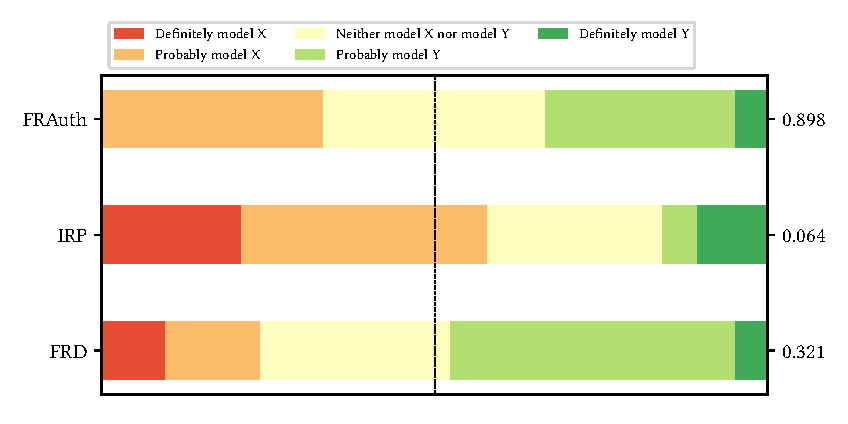
\includegraphics[width=0.8\textwidth]{figures/Q10.20/10312021/Q10.20_scenario.pdf}
    \caption{Grouped by scenario}
    \label{fig:my_label}
\end{figure}
